\pagebreak
\section{ПРОГРАММА И МЕТОДИКА ИСПЫТАНИЙ}
\label{sec:testing}

В данном разделе большее внимание уделим задачам исследования разработанной
системы с точки зрения внесенных улучшений, на что есть несколько причин.
Во-первых, В одном из модулей реализован набор программм самотестирования
ядра, во-вторых, детали реализации этих программ уже были описаны в разделе
\ref{sec:dev}, в-третьих, модуль самотестирования занимается только проверкой
корректности работы системных вызовов, но не дают информации о том, эффективно
ли их использование по сравнению с существующими интерфейсами.

Так как разработанные системные вызовы позиционируются как более быстрая замена
\texttt{procfs}, важной частью испытаний дипломного проекта является измерения
производительности разработки. Другими словами, в качестве одного из результатов
необходимо получить отношение времени работы программы при использовании старого
интерфейса и нового.

Кроме того, важно показать оправданность цели разработки, то есть показать
затратность и избыточность существующей системы на реальной машине. При этом
стоит учитывать, что код ядра выполняется почти постоянно и выполняется очень
быстро, из-за чего крайне важно обеспечить максимаьлную точность измерений и
минимизировать влияние на результаты внешних факторов. Такие меры являются
важным действием при измерении характеристик работы ядра, так как уменьшают
погрешность полученных результатов.

Продемострировать затратность получения информации из файлов возможно несколькими
способами: посчетом числа и времени в необходимых системных вызовах с помощью
\texttt{strace -c}, и подсчетом времени выполнения необязательных функций
утилитой \texttt{perf}. Кроме того, важно при замере производительности
изолировать процесс от воздействия внешних факторов для повышения точности
измерений. К таким факторам относятся непостоянность частоты ЦП ввиду
автоматического подстраивания ее под текущую нагрузку, прерывания, а также
другие процессы на текущем ядре.

В первую очередь, ядро загружается с параметром \texttt{nr\_cpus=1} для нагрузки
по умолчанию только одного ядра процессами.
Отключение изменения тактовой частоты процессора можно осуществить записью
единицы в виртуальный файл
\texttt{/sys/devices/system/cpu/intel\_pstate/no\_turbo}. Записью в файлы
\texttt{/proc/irq/*/smp\_affinity} разрешается обработка прерываний только на
нулевом процессоре, после чего при утилитой \texttt{taskset} необходимый
процесс запускается на свободном процессоре.

\begin{figure}
  \centering
  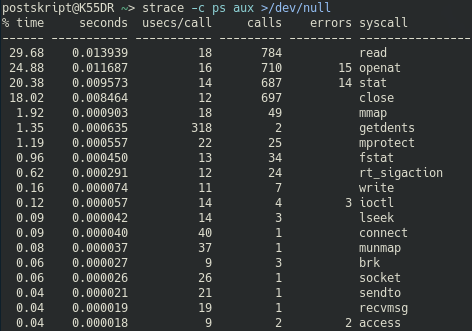
\includegraphics[width=\textwidth]{strace_ps.png}
  \caption{Получение статистики системных вызовов в ps}
  \label{fig:strace_ps}
\end{figure}

На рисунке \ref{fig:strace_ps}
продемонстрирован результат анализа выполнения команды
\texttt{strace -c ps aux}. Полученный результат
показывает, что операции, являющиеся дополнительными действиями из-за работы с
данными через виртуальные файлы и не приносящие никакой полезной информации,
могут занимать до половины времени процесса в пространстве ядра. При этом стоит
учитывать, что полученные таким способом результаты не учитывают временные
затраты на преобразования входных и выходных данных.

Результат работы профилировщика показан на рисунке \ref{fig:perf_report}.
Итоговый суммарный процент времени на дополнительные расходы равен около 20\%.
На высоконагруженных системах такая разница будет значительной, что и было
показано ранее.

\begin{figure}
  \centering
  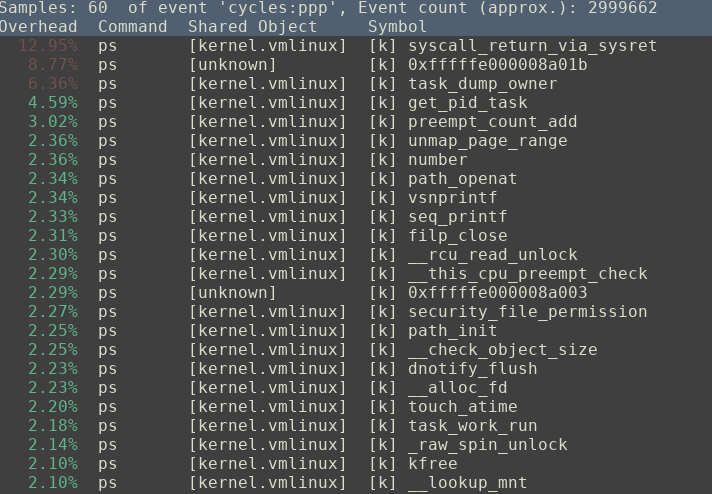
\includegraphics[width=\textwidth]{perf_report.png}
  \caption{Результат анализа производительности}
  \label{fig:perf_report}
\end{figure}

Таким образом, можно заключить, что существующий интерфейс в виде файловой
системы \texttt{procfs} является в значительной степени избыточным.

Далее рассмотрим аспекты разработки программ, измеряющих производительность
нового интерфейса и сравнивающие их с аналогичными существующими файловыми
интерфейсами.

Измерять относительное ускорение можно для нескольких условий:
\begin{itemize}
\item измерения производятся только для тех участков кода, рассмотрение которых
  ведется в данном случае (взаимозаменяемые части);
\item измеряется время работы целой программы, то есть опеределяется ускорение,
  наблюдаемое пользователем при выполнении типичных задач.
\end{itemize}

Сначала рассмотрим первый вариант. Как и любые другие тесты производительности,
разработанным программам необходимо осуществить ряд действий:
\begin{itemize}
\item подготовить среду выполнения, например, создать нужное количество файловых
  дескрипторов;
\item подготовить входные или выходные буферы, в зависимости от контекста;
\item получить начальное время исполнения;
\item выполнить измеряемые действия для одного из интерфейсов;
\item получить конечное время исполнения;
\item аккумулировать время в общий счетчик;
\item повторить узмерения определенное количество раз;
\item определить общее время в виде среднего арифметического.
\end{itemize}

После этого действия повторяются с выполнением действий при помощи другого
интерфейса. Перед всеми действиями рекомендуется выполнить описанные выше
меры по уменьшению влияния на результат внешних факторов. Пример ключевого
фрагмента одной из таких программ показан нижу, а результат работы изображен на
рисунке \ref{fig:microbench}.

\begin{figure}
  \centering
  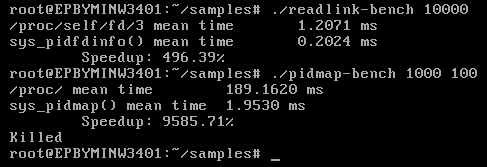
\includegraphics[width=\textwidth]{microbench.png}
  \caption{Результаты измерения производительности вызовов}
  \label{fig:microbench}
\end{figure}

\medskip
\begin{lstlisting}[style=cstyle]
int main(int argc, char *argv[])
{
	/* decls */
	fd = open(".", O_RDONLY);
	if (fd == -1) {
		perror("open");
		return 1;
	}

	/* /proc/ time */

	gettimeofday(&start, NULL);
	for (i = 0; i < count; i++)
		readlink_syscalls(fd);
	gettimeofday(&end, NULL);
	syscall_result = ((end.tv_sec  - start.tv_sec) * 1000000
			 + end.tv_usec - start.tv_usec) / (float) count;

	speedup = (float) (proc_result / syscall_result - 1.) * 100;

	printf("sys_pidfdinfo() mean time\t%.4f ms\n"
		"\tSpeedup: %.2f%%\n",
		syscall_result, speedup);

	close(fd);
	return 0;
}

/* readlink_proc impelentation */

inline void readlink_syscalls(int fd)
{
	char fibuf[PAGE];
	struct fdinfo *fi = (void *) fibuf;

	if (syscall(__NR_pidfdinfo, 0, fd, fi, PAGE) < 0)
		perror("pidfdinfo");
}
\end{lstlisting}
\medskip

Теперь рассмотрим методику измерения ощущаемого пользователем прироста
производительности. Наиболее простым решением в таком случае является запуск
программ-примеров с использованием \texttt{procfs} и новых системных вызовов,
измеряя время выполнения программой \texttt{time}. Как было упомянуто в разделе
\ref{sec:func}, примеры программ имеют опции для использования ими файловой
системы вместо бинарных вызовов, поэтому этим можно возпользоваться. Полученные
результаты показаны на рисунке \ref{fig:time}.

\begin{figure}
  \centering
  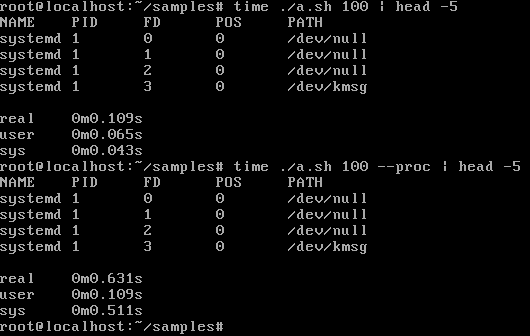
\includegraphics[width=\textwidth]{time.png}
  \caption{Результат применения бинарных вызовов}
  \label{fig:time}
\end{figure}

Таким образом, использование в пользовательских программах разработанных в
дипломном проекте системных вызовов дает ощутимый прирост производительности, в
разработанных тестовых программах только получение информации ускоряется на
500\%-10000\%, а в целом время работы типичной программы уменьшается в 6 раз.
